% Skills architecture of pstack (as bundled in nevarch).
% Build: see "Architecture" in the repository README.md
\documentclass[tikz,border=0pt]{standalone}
\usepackage[scaled]{helvet}
\renewcommand{\familydefault}{\sfdefault}
\usetikzlibrary{positioning,fit,backgrounds,arrows.meta,calc}
\pgfdeclarelayer{page}
\pgfsetlayers{page,background,main}

\definecolor{ink}{HTML}{1F2933}
\definecolor{muted}{HTML}{52606D}
\definecolor{line}{HTML}{9AA5B1}
\definecolor{userC}{HTML}{E4E7EB}
\definecolor{orchC}{HTML}{FFF3C4}  \definecolor{orchB}{HTML}{CB9D06}
\definecolor{playC}{HTML}{DCEEFB}  \definecolor{playB}{HTML}{2680C2}
\definecolor{skillC}{HTML}{E3F9E5} \definecolor{skillB}{HTML}{3F9142}
\definecolor{agentC}{HTML}{FCE8F3} \definecolor{agentB}{HTML}{B5307E}
\definecolor{cfgC}{HTML}{EAE2F8}   \definecolor{cfgB}{HTML}{724BB7}
\definecolor{distC}{HTML}{F5F7FA}

\tikzset{
  every node/.style={font=\small, text=ink},
  box/.style={draw, rounded corners=3pt, line width=0.7pt, align=center, inner sep=5pt},
  item/.style={box, fill=white, draw=#1, text width=3.9cm, minimum height=1.25cm},
  group/.style={draw=#1, rounded corners=6pt, line width=1pt, inner sep=9pt},
  title/.style={font=\bfseries\normalsize, anchor=north west, inner sep=0pt},
  arr/.style={-{Stealth[length=7pt]}, line width=1pt, draw=ink},
  dep/.style={-{Stealth[length=6pt]}, line width=0.8pt, draw=muted, dashed},
  lbl/.style={font=\footnotesize\itshape, text=muted, fill=white, inner sep=2pt},
}

\begin{document}
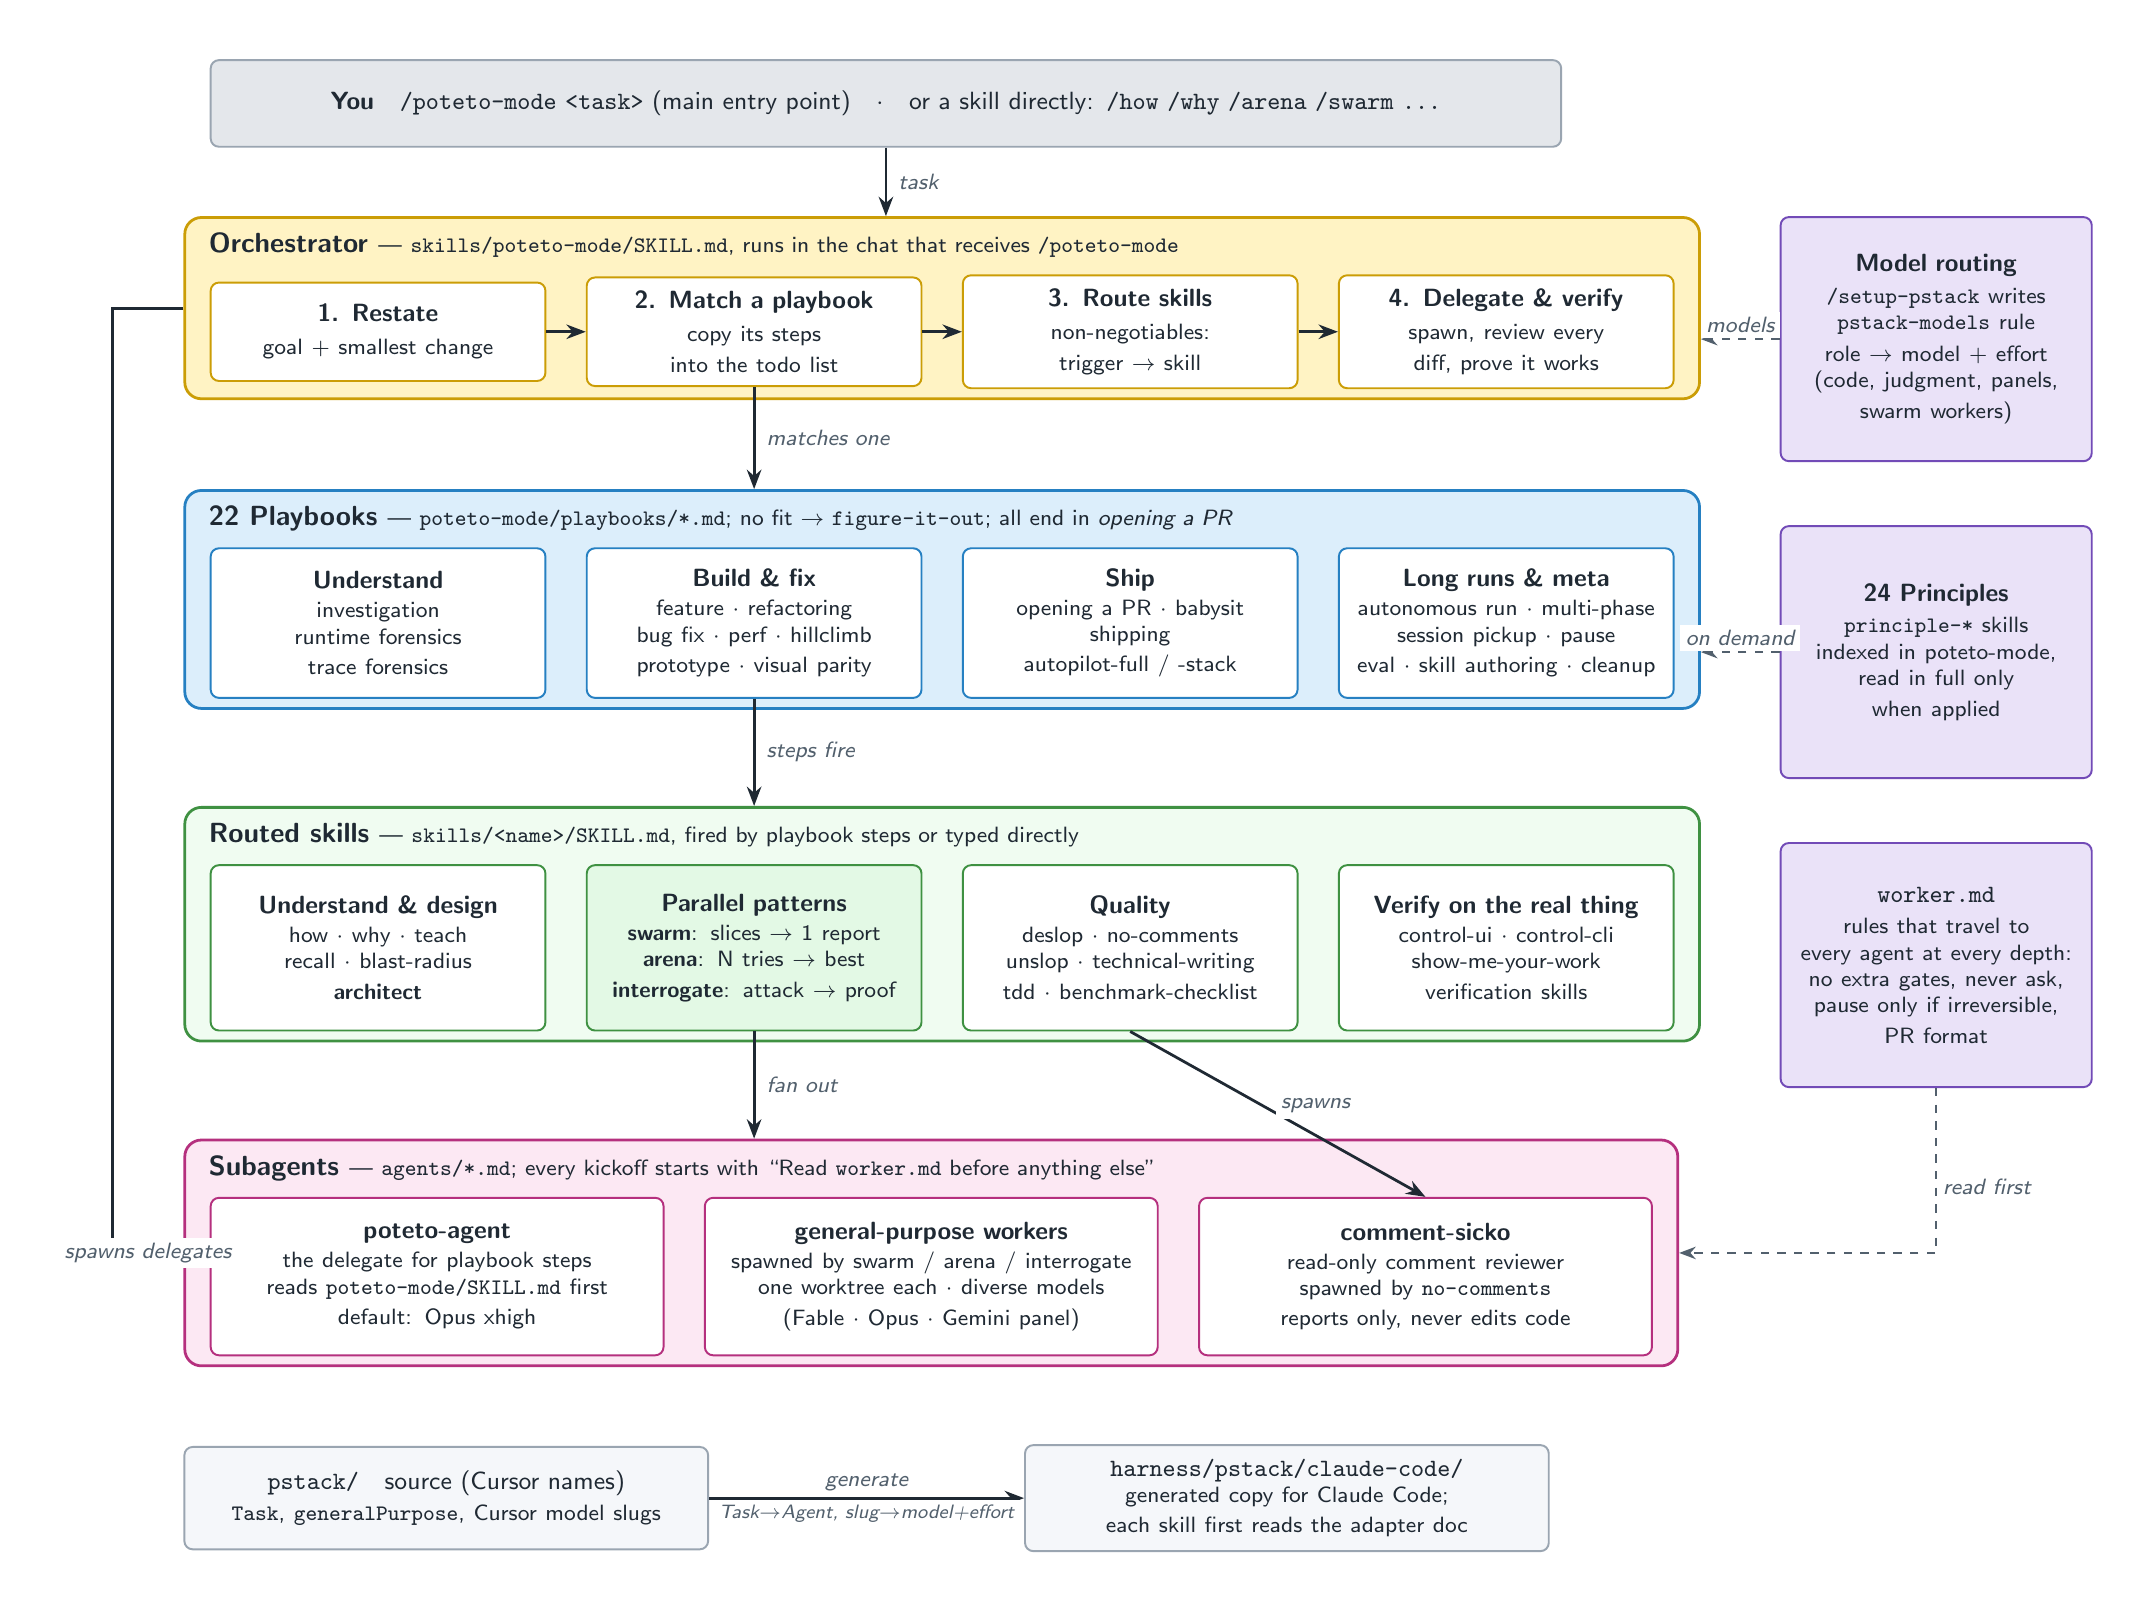
\begin{tikzpicture}[node distance=6mm and 5mm]

% ---------------------------------------------------------------- user
\node[box, fill=userC, draw=line, text width=16.8cm, minimum height=1.1cm] (user)
  {\textbf{You}\quad \texttt{/poteto-mode <task>} (main entry point)\quad$\cdot$\quad or a skill directly: \texttt{/how /why /arena /swarm \dots}};

% ---------------------------------------------------------------- orchestrator
\node[item=orchB, below=17mm of user.south west, anchor=north west] (o1)
  {\textbf{1. Restate}\\[1pt]\footnotesize goal + smallest change};
\node[item=orchB, right=of o1] (o2)
  {\textbf{2. Match a playbook}\\[1pt]\footnotesize copy its steps into the todo list};
\node[item=orchB, right=of o2] (o3)
  {\textbf{3. Route skills}\\[1pt]\footnotesize non-negotiables: trigger $\rightarrow$ skill};
\node[item=orchB, right=of o3] (o4)
  {\textbf{4. Delegate \& verify}\\[1pt]\footnotesize spawn, review every diff, prove it works};
\begin{scope}[on background layer]
  \node[group=orchB, fill=orchC, fit=(o1)(o4), yshift=3mm, inner ysep=12pt] (orch) {};
\end{scope}
\node[title] at ($(orch.north west)+(9pt,-6pt)$)
  {Orchestrator \textmd{\footnotesize --- \texttt{skills/poteto-mode/SKILL.md}, runs in the chat that receives \texttt{/poteto-mode}}};
\draw[arr] (o1) -- (o2); \draw[arr] (o2) -- (o3); \draw[arr] (o3) -- (o4);
\draw[arr] (user) -- node[lbl, right=2pt] {task} (user |- orch.north);

% ---------------------------------------------------------------- playbooks
\node[item=playB, below=21mm of o1.south west, anchor=north west, minimum height=1.9cm] (p1)
  {\textbf{Understand}\\[1pt]\footnotesize investigation\\runtime forensics\\trace forensics};
\node[item=playB, right=of p1, minimum height=1.9cm] (p2)
  {\textbf{Build \& fix}\\[1pt]\footnotesize feature $\cdot$ refactoring\\bug fix $\cdot$ perf $\cdot$ hillclimb\\prototype $\cdot$ visual parity};
\node[item=playB, right=of p2, minimum height=1.9cm] (p3)
  {\textbf{Ship}\\[1pt]\footnotesize opening a PR $\cdot$ babysit\\shipping\\autopilot-full / -stack};
\node[item=playB, right=of p3, minimum height=1.9cm] (p4)
  {\textbf{Long runs \& meta}\\[1pt]\footnotesize autonomous run $\cdot$ multi-phase\\session pickup $\cdot$ pause\\eval $\cdot$ skill authoring $\cdot$ cleanup};
\begin{scope}[on background layer]
  \node[group=playB, fill=playC, fit=(p1)(p4), yshift=3mm, inner ysep=12pt] (play) {};
\end{scope}
\node[title] at ($(play.north west)+(9pt,-6pt)$)
  {22 Playbooks \textmd{\footnotesize --- \texttt{poteto-mode/playbooks/*.md}; no fit $\rightarrow$ \texttt{figure-it-out}; all end in \emph{opening a PR}}};
\draw[arr] (o2) -- node[lbl, right=2pt] {matches one} (o2 |- play.north);

% ---------------------------------------------------------------- routed skills
\node[item=skillB, below=21mm of p1.south west, anchor=north west, minimum height=2.1cm] (s1)
  {\textbf{Understand \& design}\\[1pt]\footnotesize how $\cdot$ why $\cdot$ teach\\recall $\cdot$ blast-radius\\\textbf{architect}};
\node[item=skillB, right=of s1, minimum height=2.1cm, fill=skillC] (s2)
  {\textbf{Parallel patterns}\\[1pt]\footnotesize \textbf{swarm}: slices $\rightarrow$ 1 report\\\textbf{arena}: N tries $\rightarrow$ best\\\textbf{interrogate}: attack $\rightarrow$ proof};
\node[item=skillB, right=of s2, minimum height=2.1cm] (s3)
  {\textbf{Quality}\\[1pt]\footnotesize deslop $\cdot$ no-comments\\unslop $\cdot$ technical-writing\\tdd $\cdot$ benchmark-checklist};
\node[item=skillB, right=of s3, minimum height=2.1cm] (s4)
  {\textbf{Verify on the real thing}\\[1pt]\footnotesize control-ui $\cdot$ control-cli\\show-me-your-work\\verification skills};
\begin{scope}[on background layer]
  \node[group=skillB, fill=skillC!55, fit=(s1)(s4), yshift=3mm, inner ysep=12pt] (skills) {};
\end{scope}
\node[title] at ($(skills.north west)+(9pt,-6pt)$)
  {Routed skills \textmd{\footnotesize --- \texttt{skills/<name>/SKILL.md}, fired by playbook steps or typed directly}};
\draw[arr] (p2) -- node[lbl, right=2pt] {steps fire} (p2 |- skills.north);

% ---------------------------------------------------------------- subagents
\node[item=agentB, below=21mm of s1.south west, anchor=north west, text width=5.4cm, minimum height=2.0cm] (a1)
  {\textbf{poteto-agent}\\[1pt]\footnotesize the delegate for playbook steps\\reads \texttt{poteto-mode/SKILL.md} first\\default: Opus xhigh};
\node[item=agentB, right=of a1, text width=5.4cm, minimum height=2.0cm] (a2)
  {\textbf{general-purpose workers}\\[1pt]\footnotesize spawned by swarm / arena / interrogate\\one worktree each $\cdot$ diverse models\\(Fable $\cdot$ Opus $\cdot$ Gemini panel)};
\node[item=agentB, right=of a2, text width=5.4cm, minimum height=2.0cm] (a3)
  {\textbf{comment-sicko}\\[1pt]\footnotesize read-only comment reviewer\\spawned by \texttt{no-comments}\\reports only, never edits code};
\begin{scope}[on background layer]
  \node[group=agentB, fill=agentC, fit=(a1)(a3), yshift=3mm, inner ysep=12pt] (agents) {};
\end{scope}
\node[title] at ($(agents.north west)+(9pt,-6pt)$)
  {Subagents \textmd{\footnotesize --- \texttt{agents/*.md}; every kickoff starts with ``Read \texttt{worker.md} before anything else''}};
\draw[arr] (s2) -- node[lbl, right=2pt] {fan out} (s2 |- agents.north);
\draw[arr] (s3.south) -- node[lbl, right=4pt, pos=0.45] {spawns} (a3.north);

% o4 -> poteto-agent: route down the left margin
\coordinate (lm) at ($(orch.west)+(-0.9,0)$);
\draw[arr] (orch.west) -- (lm) |- node[lbl, pos=0.75] {spawns delegates} (agents.west);

% ---------------------------------------------------------------- side columns
\node[box, fill=cfgC, draw=cfgB, text width=3.6cm, anchor=north west, minimum height=3.1cm]
  (cfg) at ($(orch.north east)+(1.0,0)$)
  {\textbf{Model routing}\\[2pt]\footnotesize \texttt{/setup-pstack} writes\\\texttt{pstack-models} rule\\[2pt]role $\rightarrow$ model + effort\\(code, judgment, panels,\\swarm workers)};
\node[box, fill=cfgC, draw=cfgB, text width=3.6cm, below=8mm of cfg, minimum height=3.2cm] (pr)
  {\textbf{24 Principles}\\[2pt]\footnotesize \texttt{principle-*} skills\\indexed in poteto-mode,\\read in full only\\when applied};
\node[box, fill=cfgC, draw=cfgB, text width=3.6cm, below=8mm of pr, minimum height=3.1cm]
  (wk)
  {\textbf{\texttt{worker.md}}\\[2pt]\footnotesize rules that travel to\\every agent at every depth:\\no extra gates, never ask,\\pause only if irreversible,\\PR format};
\draw[dep] (cfg.west) -- node[lbl, above] {models} (orch.east |- cfg.west);
\draw[dep] (pr.west) -- node[lbl, above] {on demand} (play.east |- pr.west);
\draw[dep] (wk.south) |- node[lbl, pos=0.3, right] {read first} (agents.east);

% ---------------------------------------------------------------- distribution band
\node[box, fill=distC, draw=line, below=10mm of agents.south west, anchor=north west, text width=6.3cm, minimum height=1.3cm] (src)
  {\textbf{\texttt{pstack/}}\quad source (Cursor names)\\\footnotesize \texttt{Task}, \texttt{generalPurpose}, Cursor model slugs};
\node[box, fill=distC, draw=line, right=4.0cm of src, text width=6.3cm, minimum height=1.3cm] (cc)
  {\textbf{\texttt{harness/pstack/claude-code/}}\\\footnotesize generated copy for Claude Code;\\each skill first reads the adapter doc};
\draw[arr] (src) -- node[lbl, above] {generate} node[lbl, below, font=\scriptsize\itshape] {Task$\rightarrow$Agent, slug$\rightarrow$model+effort} (cc);

% white page so the SVG reads in GitHub dark mode too
\begin{pgfonlayer}{page}
  \fill[white] ($(current bounding box.south west)+(-0.4,-0.4)$) rectangle ($(current bounding box.north east)+(0.4,0.4)$);
\end{pgfonlayer}

\end{tikzpicture}
\end{document}
